\documentclass[c]{beamer}
\usetheme{default}
\title{Generalizing Nondeterminism for Algebraic Computation Machines}
\subtitle{Possible Subtitle}
\author{Scott Sanderson}
\institute{Department of Mathematics\\Williams College}
\date{\today}
\usepackage{tikz}
\usepackage{beamerthesiscommands}
\usepackage{mydiagrams}
\usepackage{graphicx}
\usepackage{algorithm}
\usepackage{algorithmicx}
\usepackage{algpseudocode}
\renewcommand{\algorithmicrequire}{\textbf{Input:}}
% \usepackage{enumitem}
\usetikzlibrary{calc,arrows,shapes,positioning}

\begin{document}

\theoremstyle{definition}
\newtheorem{proposition}{Proposition}
\newtheorem{proofidea}{Proof Idea}

% \begin{frame}
%   \titlepage
% \end{frame}

% \begin{frame}{Complexity Theory}
  
%   \begin{columns}
%     \visible<1->{
%       \column{0.5\textwidth}
%       \begin{figure}[h]
%         \centering \scaletopagewidth{\algoyesno{}}
%       \end{figure}
%     }
%     \visible<2->{
%       \column{0.6\textwidth}
%       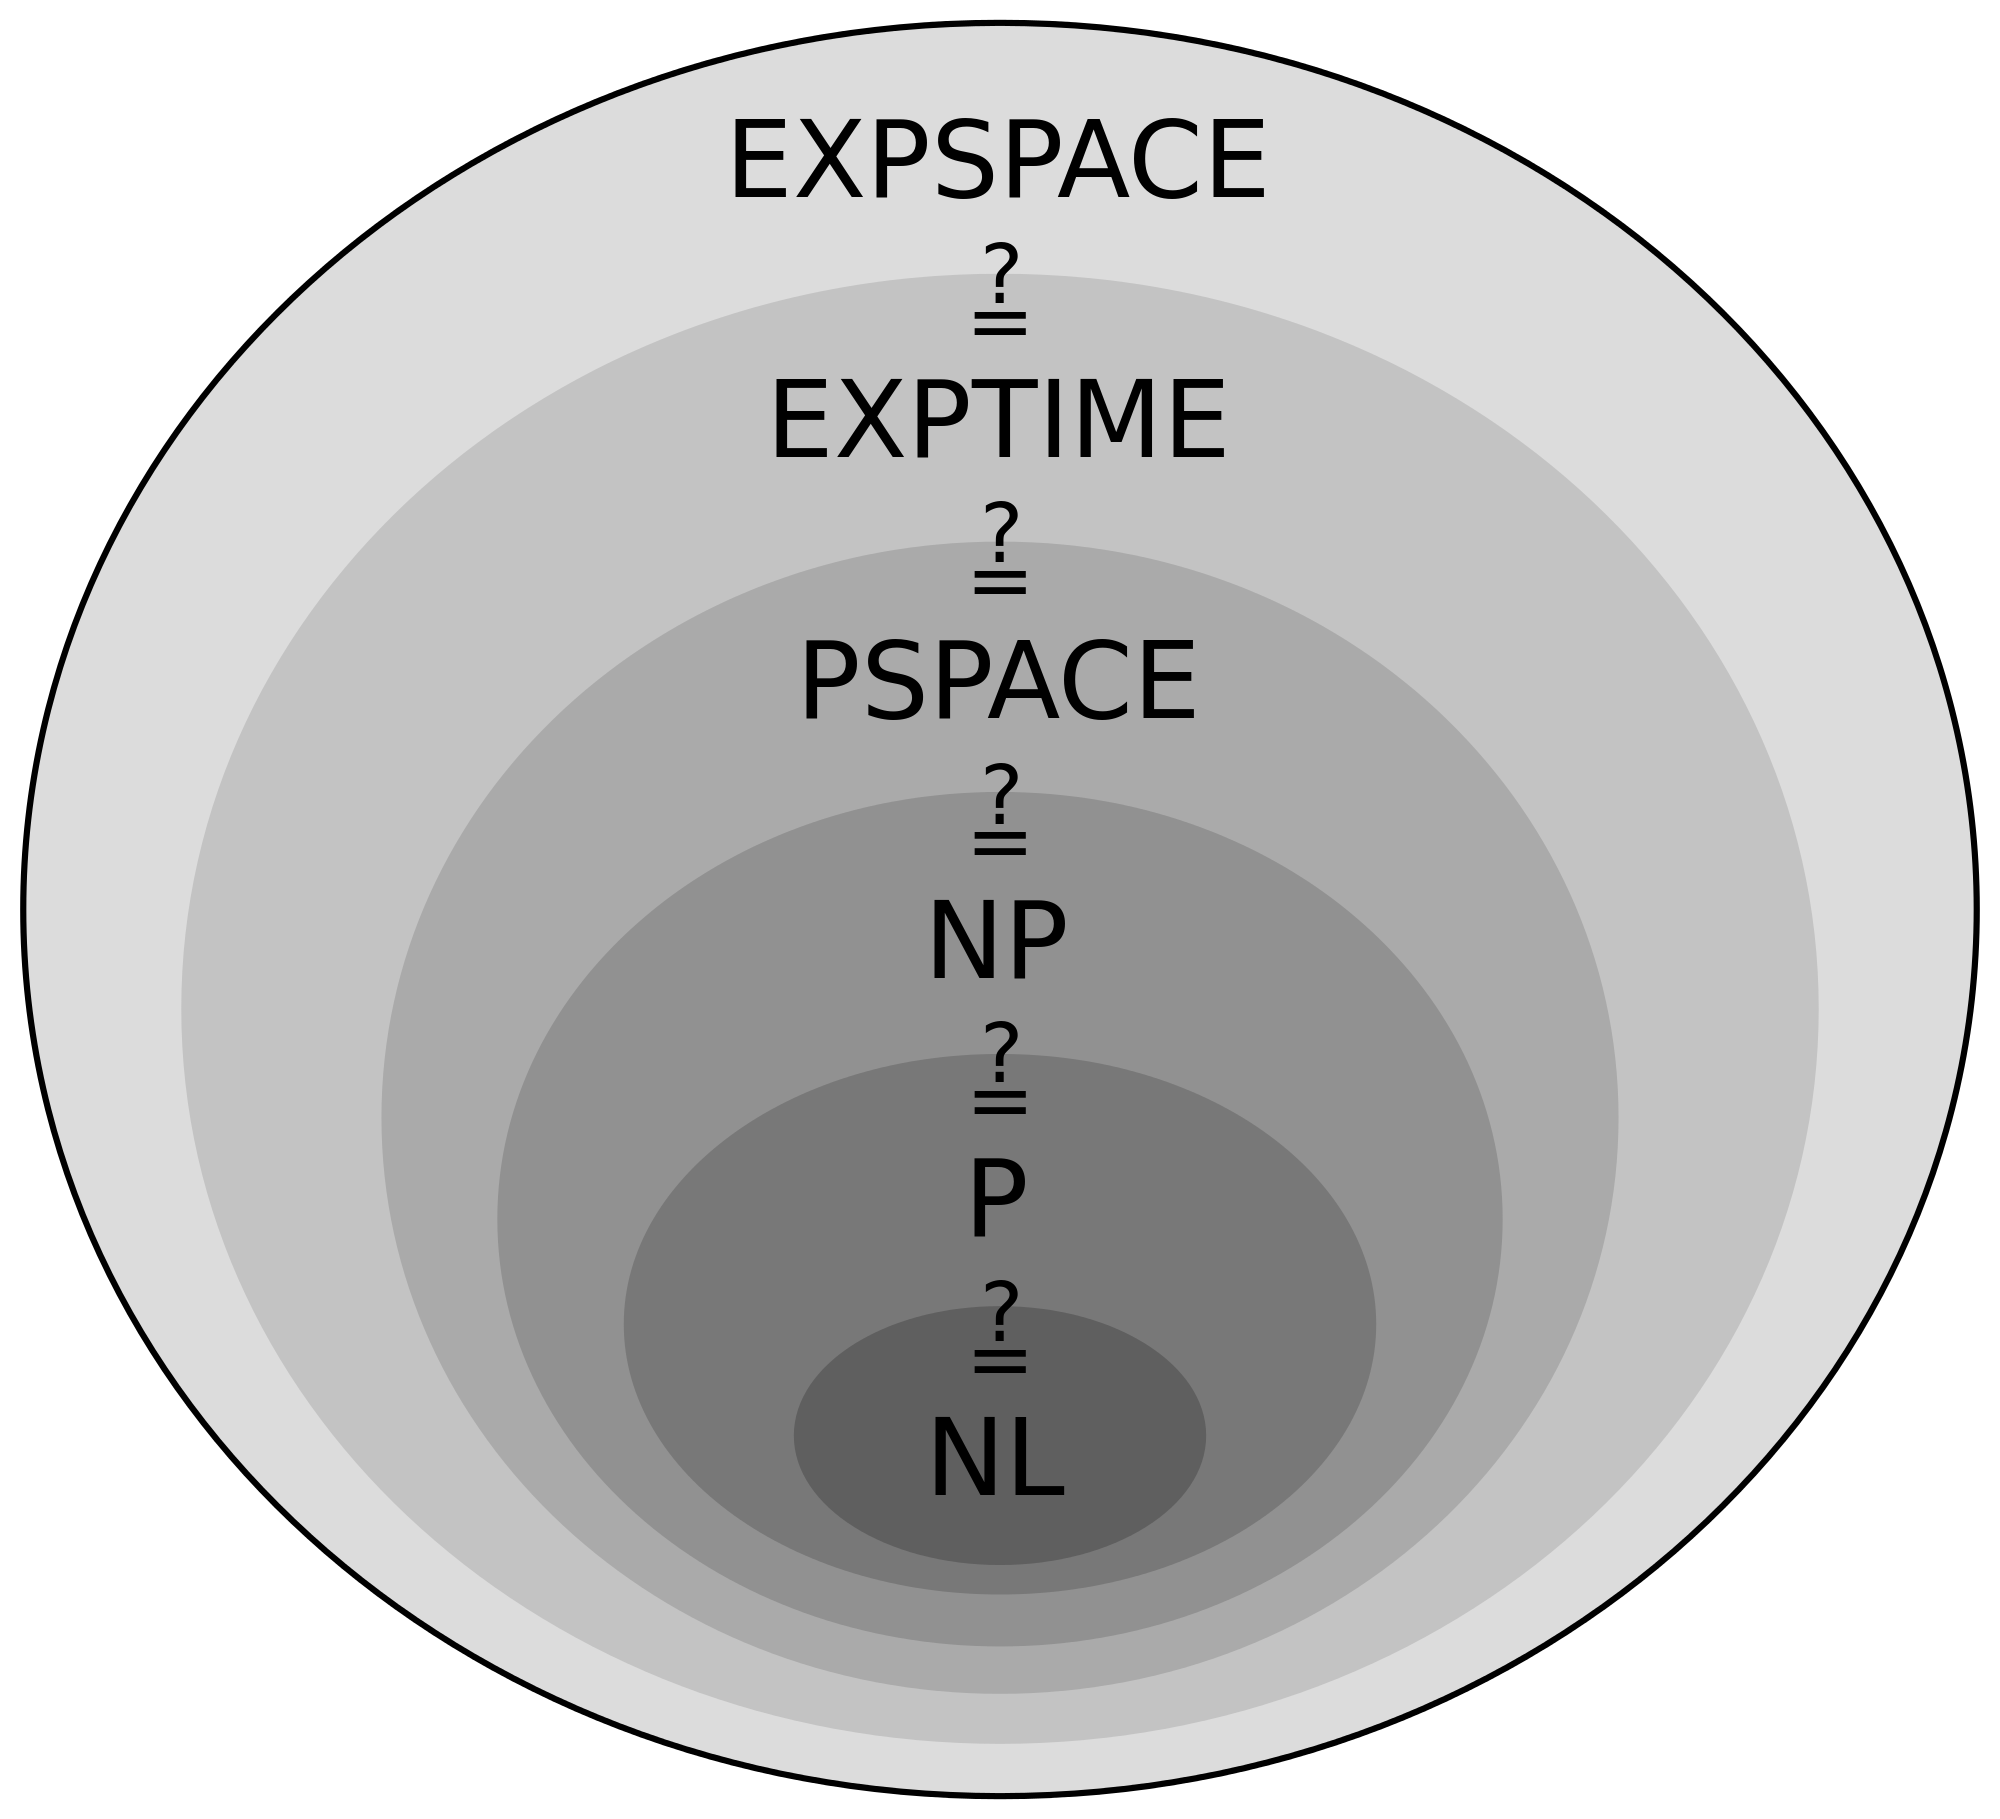
\includegraphics[width=\textwidth]{media/complexity.png}    
%     }
%   \end{columns}

% \end{frame}

% \begin{frame}{A Simple Puzzle}
  
%   \begin{itemize}
%   \item[] Does the set: $\set{1,4,7,-5,-3,18,-6,12}$ contain
%     a subset adding up to 10? \pause
%   \item[] Yes.  \textbf{Proof}: $18 - 3 - 6 + 1 = 10$ \pause
%   \item[] Does $\set{1, 17, 25, -3, 11, -9, 22, 13}$ contain a subset
%     adding up to 7?\pause
%   \item[] No.  \textbf{Proof}: Err...try them all? 
%   \end{itemize}
  
% \end{frame}

% \begin{frame}{\subsum{}}

%   An \textbf{instance} of \subsum{} is a pair $(S, t)$, where:

%     \begin{itemize}
%     \item $S = \set{s_1, s_2, \ldots, s_n}$ is a set of integers.
%     \item $t$ is a single integer, called the \textbf{target} for $S$.
%     \end{itemize}\pause

%     \vspace{\baselineskip}

%     An instance of \subsum{} is a \textbf{Yes Instance} if
%     there exists some $X \subseteq S$ such that $\sum_X = t$.\\
    
%     Otherwise it is a \textbf{No Instance}.
% \end{frame}

% \begin{frame}{Decision Problems}

%   \begin{itemize}
%   \item[] \subsum{} is an example of a \textbf{Decision Problem}.\pause
%   \item[] A Decision Problem $D$ is a set of strings,
%     partitioned into Yes Instances and No Instances, $D_{yes}$ and
%     $D_{no}$.\pause
%   \item[] Computational Complexity Theory seeks to study the intrinsic
%     \textbf{difficulty} of solving these tasks.
%   \end{itemize}

% \end{frame}

% % \begin{frame}{Machine Models}
  
% %   \begin{itemize}
% %   \item We formalize the notion of ``procedure for performing a task''
% %     by developing models of computing machines.\pause
% %   \item In classical theory of computation, the de facto machine model
% %     is the Turing Machine.
% %   \end{itemize}

% % \end{frame}

% \begin{frame}{Turing Machines}
%   \begin{columns}

%     \column{0.5\textwidth}
%     \begin{itemize}
%     \item[] Infinite one-dimensional tape, divided into cells.    
%     \end{itemize}
%     \column{0.5\textwidth}
%     \scaletopagewidth{\tape{$q$}{{1,0,1,0,0,$\blank$, $\blank$, $\cdots$}}}
%   \end{columns}
% \end{frame}

% \begin{frame}{Turing Machines}
%   \begin{columns}

%     \column{0.5\textwidth}
%     \begin{itemize}
%     \item At each step, tape head reads a symbol, writes a symbol,
%       moves left/right, and changes state.
%     \end{itemize}
    
%     \column{0.5\textwidth}
%     \scaletopagewidth{\tape[1]{$q$}{{1,0,1,0,0,$\blank$, $\blank$, $\cdots$}}}
%     $$\delta(q, 1) = (q', 0, \rightarrow)$$
%     \scaletopagewidth{\tape[2]{$q'$}{{0,0,1,0,0,$\blank$, $\blank$, $\cdots$}}}
%   \end{columns}
% \end{frame}

% \begin{frame}{Turing Machines}
%   \begin{columns}

%     \column{0.5\textwidth}
%     \begin{itemize}
%     \item Tape head instructions encoded in the machine's
%       \textbf{transition function}, $\delta$.
%     \end{itemize}
%     \column{0.5\textwidth}
%     \scaletopagewidth{\tape[2]{$q'$}{{0,0,1,0,0,$\blank$, $\blank$, $\cdots$}}}
%     $$\delta(q', 0) = (q', 1, \rightarrow)$$
%     \scaletopagewidth{\tape[3]{$q'$}{{0,1,1,0,0,$\blank$, $\blank$, $\cdots$}}}
%   \end{columns}
% \end{frame}

% \begin{frame}{Turing Machines}
%   \begin{columns}

%     \column{0.5\textwidth}
%     \begin{itemize}
%     \item Computation ends when we enter special states $q_{accept}$
%       or $q_{reject}$.
%     \end{itemize}
%     \column{0.5\textwidth}
%     \scaletopagewidth{\tape[3]{$q'$}{{0,1,1,0,0,$\blank$, $\blank$, $\cdots$}}}
%     $$\delta(q', 1) = (q_{acc}, 1, \leftarrow)$$
%     \scaletopagewidth{\tape[2]{$q_{acc}$}{{0,1,1,0,0,$\blank$, $\blank$, $\cdots$}}}
%   \end{columns}
% \end{frame}

% \begin{frame}{Turing Machine (Formal Definition)}

%   \begin{definition}[Turing Machine (TM)]

%     A \textbf{Turing Machine} is a 7-tuple, $(Q, \Sigma, \Gamma,
%     \delta, q_0, q_{accept}, q_{reject})$, where:

%     \begin{itemize}
%     \item $Q$ is a set of machine states.
%     \item $\Sigma$ is an alphabet of input characters, not containing
%       the blank symbol, $\blank$.
%     \item $\Gamma$ is the tape alphabet, with $\blank \in \Gamma$, and
%       $\Sigma \subset \Gamma$.
%     \item \functype{\delta}{(Q \times \Gamma)}{(Q \times \Gamma \times
%         \set{\leftarrow, \rightarrow})} is the machine's transition
%       function.
%     \item $q_0 \in Q$ is the initial state of the machine.
%     \item $q_{accept} \in Q$ is the machine's accept state.
%     \item $q_{reject} \in Q$ is the machine's reject state.
%     \end{itemize}
%   \end{definition}
  
% \end{frame}

% \begin{frame}{Turing Machine Example - Even or Odd?}
%   \begin{columns}[c]
    
%     \small

%     \column{0.5\textwidth}

%     \begin{itemize}
%     \item[] $Q = \set{q_0, q_1, q_{acc}, q_{rej}}$
%     \item[] $\Gamma = \set{\blank, 0, 1}$
%     \item[] $\Sigma = \set{0,1}$
%     \item[] $\delta(q_0, 0) = (q_0, \blank, \rightarrow)$
%     \item[] $\delta(q_0, 1) = (q_1, \blank, \rightarrow)$
%     \item[] $\delta(q_0, \blank) = (q_{acc}, \blank, \leftarrow)$
%     \item[] $\delta(q_1, 0) = (q_0, \blank, \rightarrow)$
%     \item[] $\delta(q_1, 1) = (q_1, \blank, \rightarrow)$
%     \item[] $\delta(q_1, \blank) = (q_{rej}, \blank, \leftarrow)$
%     \end{itemize}

%     \column{0.5\textwidth}
    
%       \scaletopagewidth[0.8]{\tape[1]{$q_0$}{{1,0,1,0,$\blank$,$\cdots$}} \vspace{1mm}}
%       \scaletopagewidth[0.8]{\tape[2]{$q_1$}{{$\blank$,0,1,0,$\blank$,$\cdots$}} \vspace{1mm}}
%       \scaletopagewidth[0.8]{\tape[3]{$q_0$}{{$\blank$,$\blank$,1,0,$\blank$,$\cdots$}} \vspace{1mm}}
%       \scaletopagewidth[0.8]{\tape[4]{$q_1$}{{$\blank$,$\blank$,$\blank$,0,$\blank$,$\cdots$}} \vspace{1mm}}
%       \scaletopagewidth[0.8]{\tape[5]{$q_0$}{{$\blank$,$\blank$,$\blank$,$\blank$,$\blank$,$\cdots$}} \vspace{1mm}}
%       \scaletopagewidth[0.8]{\tape[4]{$q_{acc}$}{{$\blank$,$\blank$,$\blank$,$\blank$,$\blank$, $\cdots$}} \vspace{1mm}}
      
%   \end{columns}
% \end{frame}

% \begin{frame}{Turing Machine Example - Even or Odd?}
%   \begin{columns}[c]
    
%     \small

%     \column{0.5\textwidth}

%     \begin{itemize}
%     \item[] $Q = \set{q_0, q_1, q_{acc}, q_{rej}}$
%     \item[] $\Gamma = \set{\blank, 0, 1}$
%     \item[] $\Sigma = \set{0,1}$
%     \item[] $\delta(q_0, 0) = (q_0, \blank, \rightarrow)$
%     \item[] $\delta(q_0, 1) = (q_1, \blank, \rightarrow)$
%     \item[] $\delta(q_0, \blank) = (q_{acc}, \blank, \leftarrow)$
%     \item[] $\delta(q_1, 0) = (q_0, \blank, \rightarrow)$
%     \item[] $\delta(q_1, 1) = (q_1, \blank, \rightarrow)$
%     \item[] $\delta(q_1, \blank) = (q_{rej}, \blank, \leftarrow)$
%     \end{itemize}

%     \column{0.5\textwidth}
    
%       \scaletopagewidth[0.8]{\tape[1]{$q_0$}{{1,0,0,1,$\blank$,$\cdots$}} \vspace{1mm}}
%       \scaletopagewidth[0.8]{\tape[2]{$q_1$}{{$\blank$,0,0,1,$\blank$,$\cdots$}} \vspace{1mm}}
%       \scaletopagewidth[0.8]{\tape[3]{$q_0$}{{$\blank$,$\blank$,0,1,$\blank$,$\cdots$}} \vspace{1mm}}
%       \scaletopagewidth[0.8]{\tape[4]{$q_0$}{{$\blank$,$\blank$,$\blank$,1,$\blank$,$\cdots$}} \vspace{1mm}}
%       \scaletopagewidth[0.8]{\tape[5]{$q_1$}{{$\blank$,$\blank$,$\blank$,$\blank$,$\blank$,$\cdots$}} \vspace{1mm}}
%       \scaletopagewidth[0.8]{\tape[4]{$q_{rej}$}{{$\blank$,$\blank$,$\blank$,$\blank$,$\blank$, $\cdots$}} \vspace{1mm}}
      
%   \end{columns}
% \end{frame}

% \begin{frame}{Limitations of Turing Machines}

%   \begin{itemize}
%   \item[] Inputs must be symbolically representable.
%   \item[] Can't talk about problems defined over $\reals$ or
%     $\complexes$.
%   \end{itemize}
  
% \end{frame}

% \begin{frame}{\subsum{} Version 2.0}
  
%   \begin{itemize}
%   \item[] Does the set $\set{1,\frac{3}{4},\sqrt{2},-5,-3,18,-6,12}$
%     contain a subset adding up to $\pi$?\pause
%   \item[] No. \textbf{Proof}: Set contains only algebraic numbers, but
%     $\pi$ is transcendental.
%   \end{itemize}
% \end{frame}

% \begin{frame}{The Mandelbrot Set $\mathcal{M}$}
  
%   Let $c \in \complexes$, we define:
%     \begin{align*}
%       p_c(z) &= z^2 + c\\
%       p_c^n(z) &= p_c(\ldots(p_c(p_c(z)))) \text{ $n$ times }\\
%     \end{align*}
    
%     \vspace{-\baselineskip}
    
%     The Mandelbrot Set $\mathcal{M}$ is given by:
%     $$\set{c \in \complexes |p_c^n(0) \nrightarrow \infty \text{ as } n \rightarrow \infty}$$
    
% \end{frame}

% \begin{frame}{The Mandelbrot Set $\mathcal{M}$}

%   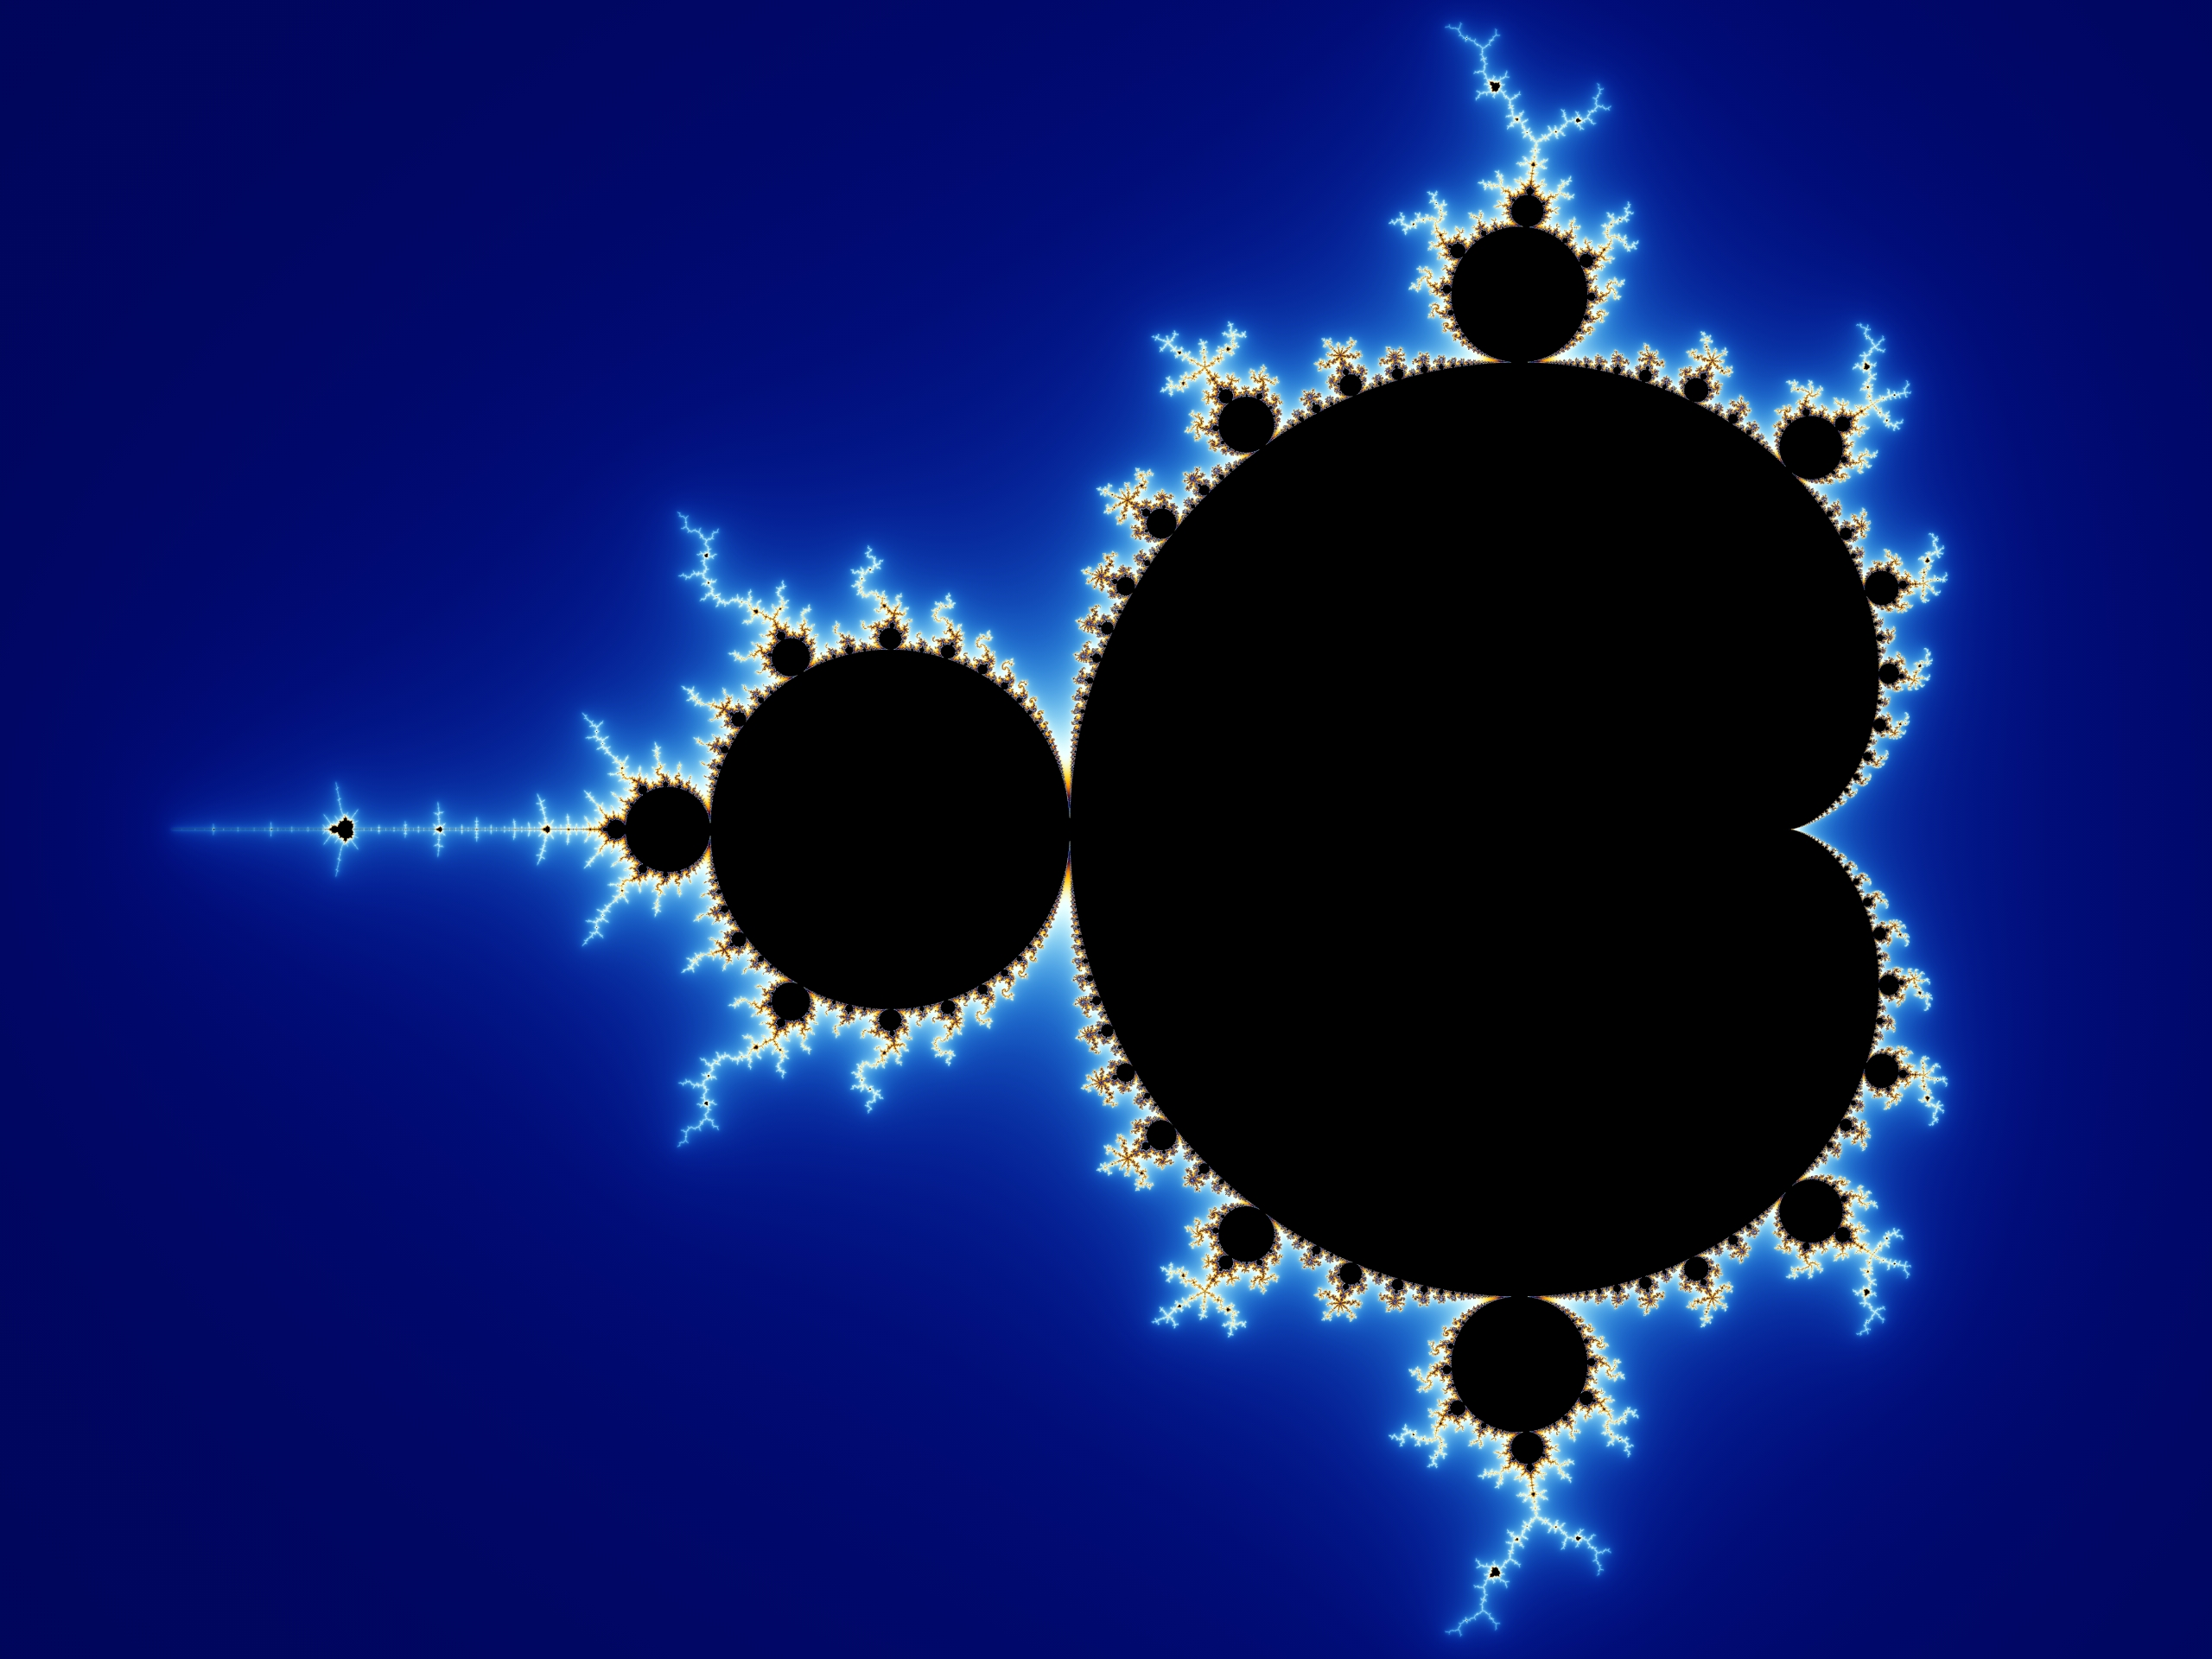
\includegraphics[width=\textwidth]{media/mandelbrot.jpg}
  
% \end{frame}

% \begin{frame}{The Mandelbrot Set as Decision Problem}
  
%   \begin{itemize}
%   \item[] In general it's ``easy'' to tell if some $c \in \complexes$ is
%     \textbf{not} in the Mandelbrot Set.\pause
%   \item[] Compute the sequence $p_c(0), p_c(p_c(0)), \ldots, p_c^n(0),
%     \ldots$. If we ever see a value with magnitude greater than 2, $c
%     \notin \mathcal{M}$.  This is \textbf{guaranteed} to happen for
%     any $c \notin \mathcal{M}$ \pause
%   \end{itemize}
% \end{frame}

% \begin{frame}{The Mandelbrot Set $\mathcal{M}$}
%   \begin{columns}

%     \column[c]{0.3\textwidth}
%     {\scriptsize
%       \textbf{Input:} $c = 0.5 + 0.5i$
%     \begin{align*}
%       p_c(0) &=& 0.5 + 0.5i\\
%       p_c(p_c(0)) &=& 0.5 + i\\
%       p_c(p_c(p_c(0))) &=& -.25 + 1.5i\\
%       p_c^4(0) &=& -1.687 + -.25i\\
%       p_c^5(0) &=& 3.285 + 1.34i\\
%     \end{align*}
%     }
%     \column{0.7\textwidth}
%     \begin{center}
%       \scaletopagewidth{
%         \begin{tikzpicture}[>=stealth]
%           \draw [thick] (-3.0,0) -- (3.0,0); 
%           \draw [thick](0,-3.0) --  (0,3.0); 
%           \draw (0,0) circle (2.0cm); 
%           \node (start) [mandpoint] at (0.0, 0.0) {};
%           \node (p0) [mandpoint] at (0.5, 0.5) {};
%           \node (p1) [mandpoint] at (0.5, 1) {};
%           \node (p2) [mandpoint] at (-0.25, 1.5) {};
%           \node (p3) [mandpoint] at (-1.6875, -.25) {};
%           \node (p4) [mandpoint, fill=red!100] at (3.285, 1.343) {};

%           \draw [->] (start) edge[out=45, in=270] (p0) {};
%           \draw [->] (p0) edge[out=90, in=270] (p1);
%           \draw [->] (p1) edge[out=90, in=0] (p2);
%           \draw [->] (p2) edge[out=180, in=90] (p3);
%           \draw [->] (p3) edge[out=0, in=270] (p4);

%         \end{tikzpicture}
%       }
%     \end{center}

%   \end{columns}
% \end{frame}

% \begin{frame}{The Mandelbrot Set $\mathcal{M}$}
  
%   \begin{itemize}
%   \item[] It seems harder to tell when $c$ will \textbf{not} escape to
%     infinity.\pause
%   \item[] If $p_c(0), p_c(p_c(0)), \ldots, p_c^n(0), \ldots$ ever
%     repeats, we know that $c \in \mathcal{M}$.
%   \end{itemize}
  
% \end{frame}

% \begin{frame}{The Mandelbrot Set $\mathcal{M}$}
%   \begin{columns}

%     \column[c]{0.3\textwidth}
%     {\scriptsize
%       \textbf{Input:} $c = i$
%     \begin{align*}
%       p_c(0) &=& i\\
%       p_c(p_c(0)) &=& -1 + i\\
%       p_c(p_c(p_c(0))) &=& -i\\
%       p_c^4(0) &=& -1 + i\\
%       p_c^5(0) &=& -i\\
%       &\vdots& \\
%     \end{align*}

%   }
%     \column{0.7\textwidth}
%     \begin{center}
%       \scaletopagewidth{
%         \begin{tikzpicture}[>=stealth]
%           \draw [thick] (-3.0,0) -- (3.0,0); 
%           \draw [thick](0,-3.0) --  (0,3.0); 
%           \draw (0,0) circle (2.0cm); 
%           \node (start) [mandpoint] at (0.0, 0.0) {};
%           \node (p0) [mandpoint] at (0, 1) {};
%           \node (p1) [mandpoint] at (-1, 1) {};
%           \node (p2) [mandpoint] at (0, -1) {};
%           \node (p3) [mandpoint] at (-1, 1) {};

%           \draw [->] (start) edge[out=45, in=0] (p0) {};
%           \draw [->] (p0) edge[out=135, in=90] (p1);
%           \draw [->] (p1) edge[out=270, in=180] (p2);
%           \draw [->] (p2) edge[out=135, in=0] (p3);

%         \end{tikzpicture}
%       }
%     \end{center}

%   \end{columns}
% \end{frame}

% \begin{frame}{The Mandelbrot Set $\mathcal{M}$}
  
%   \begin{itemize}
%   \item[] Not every point in $\mathcal{M}$ repeats like this.
%   \end{itemize}
  
%   \textbf{Input:} $c = .25$

%   \vspace{-\baselineskip}

%   \begin{align*}
%     p_c(0) &=& .25\\
%     p_c(p_c(0)) &=& .3125\\
%     p_c(p_c(p_c(0))) &\approx& .34766\\
%     &\vdots& \\
%     p_c^{10}(0) &\approx& .43055\\
%     p_c^{25}(0) &\approx& .46684\\
%     p_c^{100}(0) &\approx& .49069\\
%   \end{align*}
  
%   Always increases, but appears to converge to $\frac{1}{2}$.
  
% \end{frame}

% \begin{frame}{The Mandelbrot Set as Decision Problem}
  
%   \textbf{Question}: Does there exist an algorithm for determining
%   whether an arbitrary complex number $c$ is a member of
%   $\mathcal{M}$?
  
% \end{frame}

% \begin{frame}{Another (Easy) Decision Problem}
  
%   \begin{columns}
    
%     \column{0.5\textwidth}
%     Do there exist $x, y$ the following?
%     \begin{align*}
%       2x + 3y &= 5\\
%       x + y &= 2
%     \end{align*}

%     \column{0.5\textwidth}

%     \begin{center}
%       \scaletopagewidth{
%         \begin{tikzpicture}[>=stealth, ultra thick]
%           \draw [<->]      (-7.0,0) -- (7.0,0); 
%           \draw [<->]      (0,-7.0) -- (0,7.0);
%           \draw [<->]        (-5.0, 5.0) -- (5.0, -1.66);
%           \draw [<->]        (-5.0, 7.0) -- (5.0, -3.0);
%           \node [mandpoint, label={45:$(1, 1)$}] at (1.0, 1.0) {};
%         \end{tikzpicture}
%       }
%     \end{center}
%   \end{columns}
% \end{frame}


% \begin{frame}{Another (Easy) Decision Problem}
  
%   \begin{columns}
    
%     \column{0.5\textwidth}
%     Same as finding shared zeroes of:
%     \begin{align*}
%       f_1(x,y) &= 2x + 3y - 5\\
%       f_2(x,y) &= x + y - 2\\
%     \end{align*}

%     \column{0.5\textwidth}

%     \begin{center}
%       \scaletopagewidth{
%         \begin{tikzpicture}[>=stealth, ultra thick]
%           \draw [<->]      (-7.0,0) -- (7.0,0); 
%           \draw [<->]      (0,-7.0) -- (0,7.0);
%           \draw [<->]        (-5.0, 5.0) -- (5.0, -1.66);
%           \draw [<->]        (-5.0, 7.0) -- (5.0, -3.0);
%           \node [mandpoint, label={45:$(1, 1)$}] at (1.0, 1.0) {};
%         \end{tikzpicture}
%       }
%     \end{center}
%   \end{columns}
% \end{frame}

% \begin{frame}{Another (Less Easy) Decision Problem}
 
%   We can make the problem harder by increasing degrees, adding more
%   variables, and allowing more complicated coefficients.
  
%   \vspace{-\baselineskip}

%   \begin{align*}
%     p_1(x, y, z) &= 3xz^2 + 2xyz - y^2 - 2\\
%     p_2(x, y, z) &= x^3z + \sqrt{5}xyz + \pi y^2 + \frac{3}{5}\\
%     p_3(x, y, z) &= x^2y^2 - \frac{1}{2}y + y^3z^2
%   \end{align*}\pause
  
%   \textbf{Task:} Do there exist any values $(x_0, y_0, z_0) \in
%   \complexes^3$ such that $p_1(x_0, y_0, z_0) = p_2(x_0, y_0, z_0) =
%   p_3(x_0, y_0, z_0) = 0$?
  
% \end{frame}

% \begin{frame}{Hilbert's Nullstellensatz}
  
%   \begin{theorem}[Hilbert Nullstellensatz (Weak Form)]
    
%     Let $\set{p_1, p_2, \ldots p_m} \subseteq \polyn{K}$, with $K$ an
%     algebraically closed field.  The polynomials $\set{p_1, p_2,
%       \ldots, p_m}$ have no common zero if and only if there exist
%     polynomials
%     $$q_1, q_2, \ldots, q_m$$ such that
%     $$\sum_{i=1}^m p_iq_i = 1$$
    
%   \end{theorem}\pause
  
%   Similar sufficient condition results exist for polynomials over
%   $\reals$.

% \end{frame}

% \begin{frame}{Hilbert's Nullstellensatz as Decision Problem}

%   An instance of $\hn_R$ is a set 
%   $$S = \set{p_1, p_2, \ldots, p_m} \subseteq \polyn{R}$$ 
%   Such a set is a Yes Instance if there exists
%   a point $\bar{x} \in R^n$ such that $p_i(\bar{x}) = 0$ for $1 \leq i
%   \leq m$.  \\

%   If no such $\bar{x}$ exists, $S$ is a No Instance.
  
% \end{frame}

% \begin{frame}{BSS Machines}

%   \begin{itemize}
%   \item Introduced by Blum, Shub, and Smale in 1989 paper, ``On a
%     Theory of Computation and Complexity over the Real Numbers:
%     NP-Completeness, Recursive Functions, and Universal Machines''
%   \item Basic idea is to build a Turing Machine that can have
%     arbitrary real numbers on its ``tape''.
%   \item Extended by Blum, Shub, Smale and Cucker in 1998 book,
%     ``Complexity and Real Computation''.
%   \end{itemize}
  
% \end{frame}

% \begin{frame}{An Algorithm for Eliminating Values from $\mathcal{M}$}

%   \begin{columns}
%     \column{0.33\textwidth}
%     \begin{algorithmic}
%       \Require $c \in \complexes$
%       \State $z = 0$
%       \While{$|z| < 2$}
%       \State $z = z^2 +c$
%       \EndWhile
%       \State \textbf{Accept}
%     \end{algorithmic}

%     \column{0.66\textwidth}
%     \begin{center}
%       \scaletopagewidth[0.9]{\mandelrecsimple{}}
%     \end{center}
%   \end{columns}
% \end{frame}

% \begin{frame}{Finite Dimensional BSS Machines}

%   \begin{itemize}
%   \item A Finite Dimensional BSS Machine (FDM) $M$ over a ring $R$ is
%     a finite, directed graph with node set $\nodes$, along with an
%     associated \textbf{state space} $\statespace_M$ containing values
%     in $R^n$ for some $n \in \naturals$.\pause
%   \item $\nodes$ is analogous to Turing Machine's set of
%     states.
%   \item $\statespace_M$ is analogous to Turing Machine's tape.
%   \end{itemize}

% \end{frame}

% \begin{frame}{Finite Dimensional BSS Machines}
%   \begin{columns}
    
%     \column{0.5\textwidth}
%     \begin{itemize}
%     \item The set $\nodes$ has three distinguished nodes:
%       \begin{itemize}
%       \item \textbf{Input Node}: $\eta_1$
%       \item \textbf{Accept Node}: $\accept$
%       \item \textbf{Reject Node}: $\reject$
%       \end{itemize}
%     \item Input node reads the input and initializes finitely many
%       values in $\statespace_M$.
%     \item Accept and Reject nodes analogous to TM accept/reject
%       states.
%     \end{itemize}
%     \column{0.66\textwidth}
%     \begin{center}
%       \scaletopagewidth[.9]{\mandelrecpI{}}
%     \end{center}
%   \end{columns}

% \end{frame}

% \begin{frame}{Finite Dimensional BSS Machines}
  
%   \begin{columns}
    
%     \column{0.5\textwidth}
%     \begin{itemize}
%     \item Remaining nodes are either \textbf{computation} or
%       \textbf{branch} nodes.
%     \item Computation nodes mutate the statespace by calculating some
%       polynomial map \functype{g}{R^n}{R^n}.
%     \item Branch nodes make decisions by computing some nonzero
%       polynomial map \functype{h}{R^n}{R} and checking an equality/inequality.

%     \end{itemize}
%     \column{0.66\textwidth}
%     \scaletopagewidth[.9]{\mandelrecpII{}}
    
%   \end{columns}
  
% \end{frame}

\begin{frame}{Formal FDM (Co-recognizer for $\mathcal{M})$}
  
  \begin{columns}
    \column{0.5\textwidth}
    \begin{center}
      \scaletopagewidth[.9]{\mandlegend{}}
    \end{center}
    
    \column{0.7\textwidth}
    \begin{center}
      \scaletopagewidth[.9]{\mandelrecfull{}}
    \end{center}


  \end{columns}

\end{frame}

\begin{frame}{Example FDM}
  
  PLACEHOLDER (Rational recognizer over R)
 
\end{frame}

\begin{frame}{Path Decomposition Theorem}

  PLACEHOLDER (State, give proof idea, maybe talk about computation
  paths/coincidence sets?)
  
\end{frame}

\begin{frame}
  \begin{corollary}
    The Mandelbrot Set is undecidable.
  \end{corollary}
\end{frame}

\begin{frame}{``Full'' BSS Machines}

  PLACEHOLDER

\end{frame}

\end{document}